\documentclass[12pt]{article}

% -- fonts (Times Roman via TeX Gyre Termes) --
\usepackage[T1]{fontenc}
\usepackage{lmodern}
\usepackage{tgtermes}

% -- layout --
\usepackage[margin=1in]{geometry}
\usepackage{setspace}
\doublespacing

% -- line numbers --
\usepackage{lineno}
\linenumbers

% -- math --
\usepackage{amsmath}

% -- tables --
\usepackage{booktabs}

% -- figures --
\usepackage{graphicx}
% author-year citations with round brackets, as required by the journal
\usepackage[round,authoryear]{natbib}
\bibliographystyle{plainnat}

% -- hyperlinks (no colored links) --
\usepackage[colorlinks=false,hidelinks]{hyperref}

% -- breakable file paths: \path{} allows line breaks inside long
%    directory/file names, which \texttt{} cannot do --
\usepackage{url}
\urlstyle{tt}
\def\UrlBreaks{\do\/\do\_\do\-\do\.}

% -- PLOS requires "Fig" not "Figure" --
\renewcommand{\figurename}{Fig}

% ============================================================
% TITLE AND AUTHOR
% ============================================================

\title{Activation and Foreclosure: Separating Screening from Exit Costs in Codified Moral Communities}

\author{}

\date{}

\newcommand{\affiliation}{}

\date{}

\begin{document}

\maketitle
%\noindent\affiliation
\vspace{1em}

% ============================================================
% ABSTRACT
% ============================================================

\begin{abstract}
Strict communities are commonly explained by screening: costly requirements select committed members and deter free-riders. The same requirements also raise the cost of leaving, so observational evidence cannot separate selection from foreclosure. This paper separates them in an agent-based model of codified moral communities, in which agents observe conduct, sanction deviation, and decide whether to remain.

Three structural conditions govern the outcome. An enforcement apparatus forms only where conduct is observable and enforcement is rewarded; the threshold is joint, and neither condition alone suffices. Punishment then concentrates in a small cadre, but that concentration is a product of institutional design rather than of differences among agents: the top five percent of active agents deliver 0.580 of all punishment under the full privilege architecture and 0.091 without it. An active apparatus retains members only where exit is foreclosed. With exit open, no run reaches capture in any of 63 parameter cells despite an activation rate of 0.598; imposed closure raises capture to 0.889. Where the apparatus does not activate, closing the exit produces nothing.

Exit foreclosure arises from external imposition or from internal absorption with generational replacement. The mechanism is defined over structural properties rather than doctrinal content, and applies to any organization that codifies conduct and attaches standing to compliance.
\end{abstract}
\vspace{1em}\noindent\textbf{Keywords:} agent-based modeling; institutional design; norm enforcement; organizational capture; path dependence; religious organizations

\newpage

% ============================================================
% 1. INTRODUCTION
% ============================================================

\section{Introduction}

Why are strict religious groups often unusually cohesive and durable? The canonical answer begins with religious organizations as clubs that produce collective goods. In Iannaccone's account, apparently wasteful demands can make these clubs stronger: costly requirements involving dress, diet, ritual, time, and money screen out people whose low commitment would otherwise permit them to free-ride on the sacrifices of others \citep{iannaccone1988,iannaccone1992,iannaccone1994}. Those who remain redirect resources away from competing activities and toward the group, increasing both the average commitment of members and the value of membership itself. Strictness, on this view, is not organizational pathology but a solution to adverse selection and weak participation. This club-goods framework has become the dominant economic explanation of religious strictness, as reviews of the economics of religion emphasize \citep{iyer2016,carvalho2019}. It has also generated an unusually broad family of applications. Sacrifice and nontransferable religious capital help explain ultra-Orthodox Jewish education and fertility \citep{berman2000}; monitoring institutions can sustain religious production \citep{mcbride2007}; costly signals can resolve commitment problems in religious militancy \citep{bermanlaitin2008}; and veiling can operate as a commitment device that changes social interaction and marriage-market incentives \citep{carvalho2013}. Across these applications, costly observances select committed participants and align their investments with the group.

Yet the same arrangements have another face. Mechanisms that screen at entry typically also raise the cost of exit after entry. A social network concentrated inside the group is valuable to a committed member, but it is also difficult to replace after departure. An identity made inseparable from membership can deepen solidarity, but it can also make departure psychologically and socially disorganizing. Distinctive dress, diet, language, schooling, and ritual can certify commitment among insiders while isolating members from outsiders who might provide employment, friendship, marriage, or recognition. Screening and exit foreclosure are therefore the same social structure described from opposite directions. Looking inward from the organizational boundary, strictness selects and coordinates participants; looking outward from the position of a member considering departure, it degrades alternatives and makes separation costly. Case scholarship often recognizes both processes at once without analytically separating them. An analysis of the Skoptsy sect, for example, argues that high entry costs screened for devoted individuals while high exit costs reduced the viable alternatives for living outside the sect \citep{engelstein1999}. The two mechanisms can coexist, but coexistence does not establish which one accounts for durability.

That ambiguity is now a live theoretical problem rather than a terminological distinction. \citet{bok2025} observes that research on religious exit has concentrated mainly on who leaves, why they leave, and what follows, while the forms and roles of exit costs have received comparatively little systematic theorization. The systematic theorization of the exit-cost side is therefore recent relative to the mature literature on the determinants and consequences of exit. The field has a mature screening account and a newly articulated exit-cost problem, but no design that can adjudicate their relative causal force. The identification problem is plain. In observational data, screening and exit foreclosure arrive bundled together. Any strict group that persists has already selected some people willing to bear its demands and has also organized relationships, identities, and opportunities in ways that make leaving consequential. Comparing strict and lenient groups cannot recover the separate contribution of either process, because the strictness that filters entrants also transforms the outside option of those who stay. Nor can studying former members solve the problem by itself: observed leavers are selected on having overcome the very costs whose preventive effect is at issue. Without independent variation, evidence consistent with successful screening is also consistent with blocked exit.

Agent-based simulation supplies the missing instrument because it permits the two structures to be varied as distinct inputs while measuring any coupling between their effects. An experimental design can hold the observability and rewards that support enforcement constant while changing members' capacity to leave, or hold exit conditions constant while changing whether an enforcement apparatus can activate. No observational design can cleanly impose either intervention on otherwise equivalent religious communities. The strategy follows an established computational-religion program associated with Shults and Wildman: formal arguments for bringing simulation into the study of religion \citep{wildmansosis2011}, computational work linking cognition, culture, and social dynamics \citep{gorelemosshultswildman2018}, and agent-based analysis in the economics of religion \citep{iannacconemakowsky2007}. Simulation here is therefore not a substitute for historical or ethnographic evidence. It is a method for identifying structural effects that those forms of evidence necessarily observe in combination.

This paper distinguishes two structural dimensions that are separable across most of the grid and coupled at the frontier margin: whether an enforcement apparatus activates, and whether members can leave. Four findings organize the account. First, activation follows a joint threshold in code observability and the reward for enforcement; neither condition alone is sufficient. Second, institutional privilege concentrates punishment in a small cadre. Third, an active apparatus retains members only where exit is foreclosed. Fourth, foreclosure arises through external imposition or through internal absorption with generational replacement. These findings distinguish the conditions that form enforcement, retain its subjects, and concentrate coercive activity.

The concentration result also qualifies a prominent interpretation in the punishment literature. The costly-punishment tradition asks how sanctioning can arise through decentralized interaction even when punishers bear private costs. Experimental and evolutionary models show how punishment can sustain cooperation and how sanctioning behavior can spread or persist under specified population and institutional conditions \citep{fehrgachter2000,boydgintisbowles2010,hauertetal2007}. From that perspective, a skewed distribution of punishment may look like an emergent product of heterogeneous strategies, repeated interaction, or selection among decentralized actors. The ablation suggests a different interpretation for delegated architectures. When one role enjoys exclusive or strongly asymmetric authority, lower costs and risks, and material reinforcement, concentrated sanctioning is substantially built into the opportunity structure before interaction generates any further inequality. This is not a general claim that punishment concentration never emerges from decentralized dynamics. It is a bounded contrast: in models with an institutionally privileged enforcement role, observed concentration cannot be treated as evidence of decentralized emergence without first removing or measuring the privileges that allocate coercive opportunities.

The mechanism is content-neutral. It is defined over structural properties: how observable a code's requirements are, what rewards attach to enforcing them, whether sanctioning authority is delegated asymmetrically, and how costly it is for a member to leave. Nothing in this definition depends on the truth, theology, or substantive moral content of a doctrine. The same logic can apply to any organization that codifies conduct and attaches status to compliance, including political movements, residential communities, firms, schools, or ideological associations. Religious regimes provide the empirical terrain because they offer the longest and richest documented record of codified conduct, costly membership, delegated moral authority, and contested exit. They also make the duality especially visible, since practices experienced as identity, discipline, and mutual commitment by some members may function as barriers to outside life for others. The paper makes no claim that codified belief tends toward coercion. Its claim is conditional and structural: where observable rules, enforcement rewards, delegated privileges, and constrained exit combine, they generate dynamics that cannot be inferred from doctrine alone.

The remainder of the paper develops the argument in four steps. The next section connects screening, exit costs, and costly punishment and derives the hypotheses. The methods section specifies the agent-based design and the independent interventions on activation, exit, and privilege. The results section presents the activation frontier, exit-closure dose-response, and privilege ablation. The conclusion states the empirical implications, limits, and tests that follow from separating selection into a group from members' capacity to leave it.

\section{Literature Positioning}

\subsection{Strictness, punishment, and exit}

The club-goods account explains strict demands as screens against free riding:
costly observances select committed participants and redirect their investments
toward collective goods \citep{iannaccone1988,iannaccone1992,iannaccone1994}.
Its applications show how nontransferable capital, monitoring, costly signals,
and visible commitments stabilize demanding organizations
\citep{berman2000,mcbride2007,bermanlaitin2008,carvalho2013}.
This account identifies selection into strict groups, but it does not by itself
identify ex post policing, the concentration of sanctioning authority, or
retention when departure is costly.

Research on punishment establishes that sanctions can sustain cooperation
\citep{fehrgachter2000,fehr2002,boyd2003,boydgintisbowles2010,hauertetal2007}
and that metanorms can stabilize enforcement \citep{axelrod1986}.
Most of these models make punishment costly to the punisher.
Institutional enforcement instead can reward sanctioners with status,
resources, and authority.
The Emperor's Dilemma shows how observable enforcement and status rewards
produce cascades \citep{centola2005}, while Scott's account of legibility
explains why standardized visible conduct is administratively tractable
\citep{scott1998}.
Neither contribution joins that activation mechanism to delegated authority
and members' outside options.

\subsection{The regime problem}

Exit, voice, and loyalty identify departure as an organizational feedback
mechanism \citep{hirschman1970}; preference falsification shows how public
compliance can diverge from private belief \citep{kuran1995}.
Work on leaving religion documents the social consequences of departure
\citep{bromley1998,cragun2011,streib2009}, while models of secularization
typically emphasize affiliation or cognitive change
\citep{gelfand2011,norenzayan2013}.
The unresolved question is whether demanding systems persist because they
select committed entrants or because they diminish viable exit.

The institutional ingredients are otherwise familiar.
Coercive monopoly and administrative penetration organize sanctioning capacity
\citep{weber1946,tilly1985,mann1986}; institutions allocate enforcement power
and generate increasing returns \citep{north1990,greif2006,greif2016,pierson2000};
and histories of legitimating agents, hisbah, and inquisitorial jurisdiction
show delegated enforcement in practice
\citep{rubin2017,cook2000,given1997,kelly1989}.
Pool-punishment models likewise distinguish delegated from peer sanctioning
\citep{hilbe2014,sigmund2010}.
The present synthesis makes code observability, enforcement reward, delegated
privilege, and exit capacity independently variable.
That separation identifies when an apparatus activates, when it retains
members, and why punishment concentrates.

% ============================================================
% 3. THEORETICAL FRAMEWORK
% ============================================================

\section{Theoretical Framework}

\subsection{Codified Moral Systems}

A codified moral system is a socially shared normative structure in which obligations, prohibitions, and membership criteria are articulated in transmissible rule-form and maintained across generations through institutional mechanisms. Religious traditions are the most historically durable instances. The framework developed here is not restricted to religion; any identity-bearing system that codifies behavioral expectations and enforces compliance falls within scope. Political ideologies with loyalty tests, revolutionary movements with purity requirements, and professional bodies with ethical codes all instantiate codification to varying degrees.

As codified systems scale beyond face-to-face interaction, they confront a structural problem: moral quality must be made legible. Internal states (intention, sincerity, compassion, detachment) are opaque to observers. Institutions that must evaluate adherence therefore face pressure to adopt observable proxies. Ritual participation, dress codes, dietary restrictions, speech markers, formal declarations, and codified behaviors become instruments of classification. This shift is not incidental. It is a functional response to the problem of monitoring at scale. But it alters the incentive structure of the system. When moral standing becomes externally classifiable, enforcement roles become structurally viable.

This transformation is a problem of code geometry: the structural configuration of a codified moral system along dimensions that jointly determine whether enforcement equilibria become reachable.

\subsection{Dimensions of Code Geometry}

Five structural dimensions characterize the enforcement landscape of a codified system. These are not evaluative. They describe the formal properties of the code, not the moral worth of any tradition.

\textbf{Legibility ($\sigma$)} refers to the degree to which compliance can be externally observed and socially verified. A system is highly legible when observers can classify adherence through visible acts (dress, attendance, dietary practice, ritual performance, verbal formulae) without privileged access to internal states. A system is low in legibility when compliance depends on dispositions that cannot be reliably assessed by third parties. Legibility determines the feasibility of monitoring.

\textbf{Substitutability} captures whether externally observable compliance can function as a sufficient condition for moral standing. In high-substitutability systems, ritual performance or formal adherence terminates moral evaluation: an agent who fulfills the visible requirements is classified as moral regardless of internal state. In low-substitutability systems, external acts are explicitly necessary but insufficient; moral status depends on interior transformation that cannot be replaced by proxy performance.

Substitutability is analytically distinct from legibility. A system may render compliance visible (high legibility) without allowing visible compliance to substitute for interior reform (low substitutability). The joint condition (high legibility and high substitutability) is what makes proxy compliance a stable strategy: agents can achieve moral standing through externally performable acts alone, and observers accept this.

In the agent-based model, the parameter $\sigma$ represents the joint legibility-substitutability axis. Formally, $\sigma$ is the weight of external compliance ($s_i$) relative to internal cultivation ($x_i$) in the perceived moral score: $m_i = (1 - \sigma)x_i + \sigma s_i$. At low $\sigma$, moral evaluation depends on internal states that are opaque to observers; monitoring is infeasible and enforcement is unrewarding. At high $\sigma$, moral evaluation terminates at visible performance; monitoring is cheap and enforcement becomes structurally viable. The model collapses legibility and substitutability into a single parameter because in most codified systems these covary: systems that make compliance externally visible also tend to accept visible compliance as sufficient for moral standing. The theoretical framework distinguishes them because they can separate (monastic behavioral codes, for instance, render compliance visible without treating external observance as sufficient for spiritual attainment). The model tests the joint condition because it is the joint condition that creates the enforcement niche. Concrete indicators of high-$\sigma$ systems include dress-code compliance, attendance records, dietary markers, public prayer performance, and verbal orthodoxy tests. Concrete indicators of low-$\sigma$ systems include meditative attainment stages, sincerity of intention, character transformation, and contemplative depth. The separate observability parameters ($v_{\text{obs}}$, $a_{\text{obs}}$) in the model handle the pure observation-accuracy dimension: $v_{\text{obs}}$ captures how reliably external compliance signals are perceived, while $a_{\text{obs}}$ captures the (typically very low) probability that internal states are observable.

\textbf{Enforcement affordance} refers to the ease with which deviations can be detected, classified, and sanctioned. Systems with binary violation categories (permitted/forbidden), well-defined infraction types, and established institutional sanction pathways possess high enforcement affordance. Systems characterized by interpretive ambiguity, graduated evaluation, and contested authority possess low enforcement affordance. High enforcement affordance reduces the per-act cost of policing.

\textbf{Centralization of adjudication} describes whether interpretive and disciplinary authority is monopolized or distributed. Under high centralization, a recognized clerical, judicial, or institutional body defines orthodoxy, controls appeals, and limits interpretive plurality. Under low centralization, multiple legitimate interpretive authorities coexist, norm enforcement is local and heterogeneous, and no single body can authoritatively define deviation. Centralization does not itself produce enforcement, but it amplifies enforcement once initiated by coordinating sanctioning across a population.

\textbf{Exit cost} refers to the social, economic, legal, and identity penalties associated with leaving or dissenting from the system. When exit cost is high (apostasy carries severe sanctions, kinship networks are internal to the community, economic livelihood depends on membership, identity foreclosure makes departure psychologically costly), disaffected members are trapped. Dissent is expressed internally rather than through departure. When exit cost is low, enforcement escalation produces fragmentation rather than compliance: members leave rather than submit. Exit cost therefore determines whether tightening leads to collapse or persistence.

\subsection{From Geometry to Regimes}

The interaction of these dimensions generates distinct structural regimes. Four are consistently observed in simulation and have historical correlates.

In the \textit{quiet regime}, legibility and enforcement affordance are low, or enforcement reward is insufficient to sustain sanctioning as an adaptive strategy. Punishment remains negligible, exit is low, and the system persists without generating an enforcement niche. The code may be codified, but its structure does not render compliance auditable or sanctioning profitable.

In the \textit{collapse regime}, legibility and enforcement affordance are high but exit cost is low. Enforcement escalation triggers departure. The population shrinks, monitoring loses targets, and the system fragments. Tightening is self-defeating.

In the \textit{capture regime}, legibility, substitutability, and enforcement affordance are jointly high and exit cost is also high. Enforcement escalation does not produce mass departure. Sanctioning stabilizes because it is rewarded: enforcers gain status, institutional access, or material benefits. Compliance becomes self-reinforcing. The system converges on an enforcement-dominated equilibrium in which visible compliance is near-universal but may coexist with private dissent.

In the \textit{mixed regime}, exit is feasible but non-trivial, and membership confers benefits sufficient to retain a substantial fraction of the population. Partial exit coexists with a hardened enforcement core. Overall prevalence may decline, but active participants exhibit higher rigidity and enforcement intensity than the pre-tightening population. The system persists in reduced form.

These regimes arise from structural incentives. They do not require abnormal psychological distributions, charismatic leaders, or exogenous political shocks, though all of these can shift parameters and change which regime the system occupies.


% ============================================================
% 4. PARAMETER-OBSERVABLE MAPPING
% ============================================================

\section{Parameter-Observable Mapping}

The results require four correspondences between model inputs and observable
institutional features.
The substitution weight \(\sigma\) represents how strongly public conduct,
rather than opaque interior states, determines perceived moral standing.
Enforcement reward \(\pi\), net of its cost \(\kappa\), represents status,
promotion, resources, or authority attached to successful sanctioning.
The privilege bundle represents an operative cadre's quota, coercive
multiplier, monopoly, protection, capital gains, patronage, and cost discount.
Exit conditions represent the relational, economic, legal, and cultural
resources that make departure practicable.

These are mappings from parameters to institutional features, not scores for
whole traditions.
The observational unit is a historically bounded regime in a specific legal
and institutional setting.
The mapping is configurational: no single value determines a regime, and the
same tradition can occupy different locations across periods or institutions.
It does not measure latent sincerity or assert that visible conduct is morally
sufficient.
It asks whether a regime treats auditable performance as a usable proxy and
whether it rewards, delegates, and retains the actors organized around that
proxy.
Online Resource 1, Section~S1, supplies the complete indicator table, parameter
defaults, tested ranges, and extended measurement justification.

% ============================================================
% 5. AGENT-BASED MODEL
% ============================================================

\section{Methods}

The model is documented here in the ODD protocol order: purpose and patterns;
entities, state variables and scales; process overview and scheduling; design
concepts; initialisation; input data; submodels. Two further subsections,
experimental design and reproducibility, follow the protocol proper and describe
the simulation experiments run on the model and the provenance of their outputs.

\subsection{Purpose and patterns}

The model asks when a highly observable behavioral code can support an
enforcement institution, and when restrictions on exit convert activated
enforcement into durable capture. It is evaluated against three patterns. First,
whether an enforcement apparatus forms at all, measured as the activation of
step-level punishment among active agents. Second, whether an activated
apparatus retains its members, measured as the terminal exit rate. Third,
whether sanctioning concentrates in a small minority, measured as the share of
punishments issued by the most active agents and as the Gini coefficient of
punishment counts. The model is judged adequate to the extent that these three
patterns respond to distinct structural inputs rather than moving together.

\subsection{Entities, state variables and scales}

The entities are individual agents embedded in a social network and a
system-level institutional controller. There is one agent class and one
controller; the enforcer cadre is a collective defined over agents rather than a
separate entity.

Each agent carries intrinsic cultivation \(x_i\), belief position \(y_i\),
literalism \(L_i\), rigidity \(b_i\), enforcement propensity \(r_i\), a binary
externally legible compliance marker \(s_i\), accumulated utility, institutional
capital, accumulated service, an enforcer flag, an exit-intent counter, a
disengagement flag, an exited flag, and its position in the network. Literalism
is a fixed trait; the remaining quantities change during a run.

The controller carries a threat level \(T_t\), an authority level \(A_t\), a
patronage budget, the current enforcement reward and punishment severity, the
heresy-distance threshold, the orthodox belief position, and the current
outside-option degradation \(\delta_t\).

Time is discrete and one step is the model's only temporal unit; the model
makes no claim about the calendar duration a step represents. Space is not
represented; the network is the only relational structure. Each reported run
begins with \(N=350\) agents and proceeds for 450 steps, the horizon encoded by
the sweep launcher and represented by 450 metric rows in each committed run.
This horizon applies to the shock factorial, delta-decoupling, exogenous
dose-response, activation-boundary, and privilege-ablation experiments. Each
experimental cell uses 30 independent seeds, numbered 1 through 30.

\subsection{Process overview and scheduling}

At the start of a step, the institutional controller applies or relaxes threat,
updates authority and the patronage budget, changes punishment reward and
severity and the heresy threshold, and, unless orthodoxy is fixed, updates the
orthodox belief position. Agents are then shuffled and update their states. The
model next recomputes mean literalism among active agents, clears and reselects
the cadre, resets punishment counters, determines whether monopoly is active,
and executes the shuffled punishment phase. It then computes active-agent
punishment incidence, distributes patronage, and updates \(\delta_t\). Finally,
agents are reshuffled and attempt exit; successful exits remove edges as
described under Submodels. The clock is incremented after exit. The outer
simulation loop records metrics immediately before each call to this ordered
step, so the committed files contain rows indexed \(t=0,\ldots,449\).

Within the agent-update, punishment, and exit phases the order of agents is
randomised afresh each step, so no agent holds a fixed position in the
within-step sequence. Updates within each phase are asynchronous: an agent acts
on the state left by agents that moved earlier in the same phase.

\subsection{Design concepts}

\paragraph{Basic principles.} The model combines three ideas developed
separately in the literature reviewed above: that costly, externally legible
observance screens and coordinates participants; that sanctioning becomes
self-sustaining when it is institutionally rewarded rather than privately
costly; and that the value of the outside option governs whether tightening
produces departure or compliance. Legibility is represented as a structural
property of the code rather than as a property of individuals.

\paragraph{Emergence.} Enforcement activation, the terminal exit rate, and the
distribution of punishment across agents are all outcomes of agent and
controller rules rather than imposed values. No agent begins with an enforcement
role; cadre membership is recomputed each step from accumulated capital,
literalism, and rigidity. The privilege ablation reported in the Results shows
that the concentration of punishment, although not imposed directly, is largely
allocated by the institutional privilege architecture rather than generated by
unprivileged interaction.

\paragraph{Adaptation.} Agents adapt indirectly rather than by optimisation.
Each agent chooses whether to display the visible compliance marker with a
probability that responds to the local compliance and enforcement norms among
its network neighbours, updates intrinsic cultivation through a noisy investment
decision, and accumulates or sheds exit intent according to its own utility,
the punishment it has received, its degree, and the membership reward.

\paragraph{Objectives.} The model contains no explicit objective function that
any agent maximises. Accumulated utility is a state variable that enters
probabilistic decision rules, principally the exit-desire logistic, rather than
a quantity agents are assumed to maximise.

\paragraph{Learning.} Agents update enforcement propensity \(r_i\) and rigidity
\(b_i\) within a run on the basis of punishment outcomes. A favourable outcome
raises \(r_i\) by 0.04 and \(b_i\) by 0.03; an unfavourable one lowers them by
half those amounts. Both are clipped to \([0,1]\). Literalism does not change,
so the only trait heterogeneity that persists unchanged across a run is the
literalism draw.

\paragraph{Prediction.} Agents make no explicit forecast. Decisions use current
local information only, with the tacit assumption that present local conditions
persist into the next step.

\paragraph{Sensing.} Agents observe their network neighbours imperfectly. A
compliance marker is observed with probability \(v_{\mathrm{obs}}=0.90\),
intrinsic cultivation with probability \(a_{\mathrm{obs}}=0.05\), and a belief
position, for the heresy-distance term, with probability
\(h_{\mathrm{obs}}=0.15\). Agents sense only their neighbours, not the
population. The controller senses population-level quantities directly: the
active-agent punishment incidence, mean literalism among active agents, and,
unless orthodoxy is fixed, the mean belief position of high-literalism agents.

\paragraph{Interaction.} Interaction is local and mediated by the network in the
compliance, cultivation, and punishment phases: agents perceive and sanction
network neighbours. Interaction is global through the controller, which sets the
enforcement reward, punishment severity, heresy threshold, and authority faced
by every agent, and which distributes the patronage budget among enforcers.

\paragraph{Stochasticity.} A single seeded generator drives network generation,
the initial trait draws, the imperfect observation draws, the compliance-display
and punishment probabilities, backlash realisation, the exit-desire and
exit-opportunity draws, edge removal on exit, and the per-phase shuffling of
agent order. Stochasticity represents unmodelled heterogeneity and the
unreliability of social observation. Every reported cell is replicated over 30
seeds.

\paragraph{Collectives.} Two collectives exist. The enforcer cadre is an
emergent group, cleared and reselected every step from the active population by
the ranking rule given under Submodels, with no persistent membership. The
institutional controller is an imposed collective representing the organisation
as a whole; it holds no agent state of its own beyond the controller variables
listed above.

\paragraph{Observation.} Two files are written per run. The step-level file
records one row per step with the population-level quantities used in analysis,
including punishment incidence, exit rate, threat, authority, budget, enforcer
fraction, capital and service summaries, and the current closure level. The
agent-level file records one row per agent at the end of the run, including
punishments issued and received, terminal traits, capital, service, enforcer
status, exit status and time, effective exit cost, and degree. The outcome
classification and the concentration metrics computed from these files are
defined below.

\paragraph{Outcome classification.} The finalized classifier treats activation
and retention as separate axes. A run is active when \texttt{max\_punish} is at
least 0.10 and retained when \texttt{final\_exit\_rate} is at most 0.20. Hence
\begin{equation}
 \mathrm{CAPTURE}=\mathbf{1}\{\mathrm{final\_exit\_rate}\leq0.20\}\,\mathbf{1}\{\mathrm{max\_punish}\geq0.10\}.
\end{equation}
The four cells are QUIET for inactive and retained runs, QUIET for inactive and
not-retained runs, MIXED for active and not-retained runs, and CAPTURE for
active and retained runs. COLLAPSE, defined descriptively by exit at least 0.90,
is a tail within the inactive region rather than a separate analytical regime.
In the committed data, 100 percent of collapse runs have \texttt{max\_punish}
below 0.10, so depopulation occurs without activation.

The joint robustness band for the activation threshold is \([0.075,0.15]\). At
0.05 the low-\(\sigma\), low-\(\pi\) necessity cell revives, whereas at 0.20 the
exogenous-\(\delta\) dose-response degenerates to approximately zero capture
throughout. We therefore report continuous enforcement and exit surfaces as the
primary results and use the four-class discretization as a secondary summary.
The classifier excludes an enforcer-punishment-share criterion because that
criterion changes 0 of 9,570 committed classifications.

\paragraph{Concentration and incidence metrics.} Step-level punishment incidence
is computed only among active agents. For run \(r\), \texttt{max\_punish} is the
maximum across recorded steps of the fraction of then-active agents receiving at
least one punishment in that step. \texttt{final\_exit\_rate} is the terminal
fraction of the original population whose exited indicator is true.

For the privilege ablation, let \(c_i\) be cumulative punishments issued by agent
\(i\), restricted to agents active at the end of the run, and let \(n_a\) be
their number. Then
\begin{equation}
 \mathrm{top5pct\_share\_active}=\frac{\sum_{i\in\mathcal{K}}c_i}{\sum_{i=1}^{n_a}c_i},\qquad |\mathcal{K}|=\max\{1,\lceil0.05n_a\rceil\},
\end{equation}
where \(\mathcal{K}\) contains the largest counts. With \(c_{(i)}\) sorted in
ascending order, the active-agent Gini is
\begin{equation}
 \mathrm{gini\_active}=\frac{n_a+1-2\sum_{i=1}^{n_a}\left(\sum_{j=1}^{i}c_{(j)}\right)/\sum_{j=1}^{n_a}c_{(j)}}{n_a},
\end{equation}
and is set to zero when the vector is empty or has zero total. The
random-allocation null holds the observed active-agent punishment volume and
\(n_a\) fixed, allocates events by a multinomial distribution with equal
probability \(1/n_a\), repeats this allocation 100 times using the run seed, and
records the median simulated Gini. \texttt{enforcer\_punish\_share} is reported
descriptively only. It saturates near 0.97 wherever punishment occurs and
therefore does not provide a graded or discriminating concentration measure.

\subsection{Initialisation}

Every run is initialised from its seed, so initialisation is reproducible and
varies across replicates but not across experimental conditions at a given seed.

At initialization, intrinsic cultivation is
\(x_i\sim\operatorname{clip}_{[0,1]}\{\mathcal{N}(0.35,0.12^2)\}\), belief
position is \(y_i\sim\operatorname{clip}_{[0,1]}\{\mathcal{N}(0.50,0.12^2)\}\),
and literalism is \(L_i\sim\operatorname{Beta}(1.5,4.5)\). Rigidity and
enforcement propensity are drawn independently as
\(b_i,r_i\sim\operatorname{Beta}(2,4)\). The externally legible compliance marker
begins at \(s_i=0\). Utility, institutional capital, and accumulated service
begin at zero; all agents enter as non-exited members without an enforcement
role. Agents are exchangeable draws from common initial distributions and have
no preassigned enforcement role.

The reported sweeps use a Barab\'asi--Albert scale-free network. Its attachment
parameter is
\begin{equation}
 m=\max\{2,\operatorname{round}[\log(N+1)]\}=6
\end{equation}
for \(N=350\). Network generation uses the run seed.

The controller begins with threat at zero, and therefore with authority at zero
and the patronage budget at its constant term. The closure level begins at the
imposed baseline \(\delta_0\) for the experimental cell.

\subsection{Input data}

The model uses no external input data to represent time-varying processes.
Every driver is either endogenous to the agent and controller rules or fixed by
a parameter for the duration of a run, including the threat schedule, which is a
list of step indices rather than an empirical series. No empirical dataset is
read at run time and no results reported here are calibrated to observations.

The only file read at launch is the calibration parameter set that supplies
seven model parameters to the sweep driver. It is committed at
\path{results/BEST_PARAMS_frozen.json} and its contents are given in Online
Resource 1.

\subsection{Submodels}

\paragraph{Perception and the code-geometry parameter.} The code-geometry
parameter \(\sigma\in[0,1]\) weights externally legible compliance relative to
intrinsic cultivation in the perceived-morality signal,
\begin{equation}
 \widehat m_{ij}=(1-\sigma)\widehat x_{ij}+\sigma\widehat s_{ij}.
\end{equation}
Compliance is observed with probability \(v_{\mathrm{obs}}=0.90\), whereas
cultivation is observed with probability \(a_{\mathrm{obs}}=0.05\). Failed
compliance observation is coded as zero; failed cultivation observation is
replaced by a draw from
\(\operatorname{clip}_{[0,1]}\{\mathcal{N}(0.35,0.25^2)\}\). The same geometry
enters the legibility index
\begin{equation}
 \ell(\sigma)=\sigma v_{\mathrm{obs}}+(1-\sigma)a_{\mathrm{obs}}.
\end{equation}
The enforcement-reward parameter \(\pi\) is the coefficient on this index in the
utility return to a successful punishment. If effective enforcement cost is
\(\kappa_{i,t}^{\mathrm{eff}}\), the punisher's immediate net institutional
return is
\begin{equation}
 \Delta u_{i,t}^{\mathrm{pun}}=\pi_t\ell(\sigma)-\kappa_{i,t}^{\mathrm{eff}}.
\end{equation}
The controller may raise \(\pi_t\) above its experimental baseline after a threat
shock, as described below.

\paragraph{Agent update.} During an active agent update, visible compliance is
chosen probabilistically from local compliance and enforcement norms,
cultivation is updated by a noisy investment decision, and belief drifts weakly
toward the current orthodoxy. Each active agent also receives a per-step
membership reward
\begin{equation}
 g_{i,t}=0.0634+0.08\,\ell(\sigma)+0.1055\,T_t,
\end{equation}
which is added to its utility and therefore offsets exit desire. Capital and
service decay every step at rates 0.005 and 0.02, respectively. Exited agents are
excluded from compliance and enforcement; their capital and service continue to
decay and their belief follows a small random walk.

\paragraph{Exit.} Exit has distinct desire and opportunity components. The
baseline opportunity parameter is \texttt{exit\_opportunity\_base} \(=0.30\) in
all reported experiments, and \texttt{exit\_threshold} \(=-1.0\). With degree
\(d_{i,t}\), threat \(T_t\), and current outside-option degradation \(\delta_t\),
the raw opportunity is
\begin{align}
 B_t&=\begin{cases}0.30,&\delta_t=0,\\0.30(1-\delta_t),&\delta_t>0,\end{cases}\\
 p^{\mathrm{raw}}_{i,t}&=\operatorname{logit}^{-1}(B_t-0.03d_{i,t}-2.908T_t),\\
 \widetilde p_{i,t}&=0.02+0.98\left(p^{\mathrm{raw}}_{i,t}\right)^{5.98}.
\end{align}
In legacy and exogenous modes,
\(p^{\mathrm{opp}}_{i,t}=\widetilde p_{i,t}(1-\delta_t)\) when \(\delta_t>0\); in
decoupled mode the outer factor is not applied. Exit desire is a logistic
function of the threshold minus accumulated utility, punishment received,
degree, and membership reward. Desire must accumulate for twelve steps, after
which a new opportunity draw must succeed. Effective exit cost is
\(1.00(1+0.03d_{i,t})+0.25s_i\). After a successful exit, the model samples and
removes \(\operatorname{round}(0.90d_i)\) of the exiting agent's current \(d_i\)
incident edges. Thus exit removes 90 percent of an exiting agent's edges up to
integer rounding, rather than leaving the initial network fixed.

\paragraph{Outside-option closure.} Let \(\delta_0\) denote the imposed baseline
and \(\eta\) the drift rate, clipped by the code to \([0,0.5]\). Drift is updated
only when the step-level fraction of active agents punished is at least 0.08.
Conditional on that gate,
\begin{equation}
 \delta_{t+1}=\operatorname{clip}_{[0,1]}\left\{\delta_t+\eta(\delta_t^{*}-\delta_t)\right\}.
\end{equation}
Exit capacity is specified as an independent structural input, because a
specification in which closure is driven by the enforcement activity it is meant
to explain yields capture by construction and is uninformative about it. In the
independent-input specification,
\begin{equation}
 \delta_t^{*}=\min\{\delta_{\max},\delta_0+\kappa q_t\},
\end{equation}
where \(q_t\) is the active-agent punishment incidence, \(\delta_{\max}=0.85\),
and the experiment varies \(\kappa\). In exogenous mode no drift occurs and
\(\delta_t=\delta_0\) throughout.

\paragraph{Cadre selection.} The model reselects an enforcer cadre after agent
updates in every step. Among active agents the target cadre size is
\(Q_t=\operatorname{round}(0.08N_t^{\mathrm{active}})\), with a minimum of one
when the quota fraction is positive. Agents with capital at least 0.25 are
eligible first. Eligible agents are ranked by
\begin{equation}
 z_i=0.6\,\mathrm{cap}_i+0.3L_i+0.1(r_ib_i).
\end{equation}
If fewer eligible agents exist than the quota, the remaining positions are
filled by the highest-ranked ineligible agents. Status is cleared and reassigned
each step.

\paragraph{Privilege bundle.} The full privilege bundle combines exclusivity,
differential coercive capacity, reduced costs and risks, and material
reinforcement. When controller authority \(A_t\geq0.35\), the punishment monopoly
excludes all non-enforcers from policing. When monopoly is on, the enforcer
punishment-probability multiplier is 1.5. When monopoly is off, enforcers retain
the 1.5 multiplier while non-enforcers receive the operative multiplier
\texttt{non\_enforcer\_punish\_eps} \(=0.02\). The separately declared value
\texttt{non\_enforcer\_punish\_mult} \(=0.25\) is passed by the sweeps but is not
used in this operative branch. After a punishment, capital first reduces the base
cost according to
\begin{equation}
 \kappa_{i,t}'=0.08\left(1-0.20\,\mathrm{cap}_{i,t}\right),
\end{equation}
and an enforcer pays \(0.30\kappa_{i,t}'\), a further 70 percent role discount.
Enforcer backlash probability is multiplied by 0.25, giving 75 percent protection
relative to an otherwise identical non-enforcer. Every successful punishment adds
0.15 capital, capped at 2.0, and one unit of service. The nonnegative controller
budget \(0.15+0.60T_t\) is distributed only among active enforcers: equally if
their total service is zero, otherwise in proportion to nonnegative accumulated
service. These mechanisms jointly constitute the ceiling arm of the privilege
ablation.

\paragraph{Threat controller.} At scheduled shock times \(t\in\{100,220,320\}\),
threat increases by 0.10; otherwise it decays by a factor \(1-0.03\). Authority
is \(A_t=1-\exp(-2T_t)\), the budget is \(0.15+0.60T_t\), punishment reward and
severity each rise by \(0.20T_t\) from baseline, and the heresy-distance
threshold falls by \(0.08T_t\), subject to clipping. The shock-off factorial and
all decoupled runs use an empty schedule, so threat is identically zero in those
runs and every threat-gated term above vanishes.

\subsection{Experimental design}

The shock factorial is committed at
\path{recon/factorial_shock_off/sweep_seed_results.csv} and
\path{recon/factorial_shock_on/sweep_seed_results.csv}. Each condition contains
4,050 runs from \(\eta\in\{0,\allowbreak 0.05,\allowbreak 0.10,\allowbreak
0.20,\allowbreak 0.30\}\), \(\delta_0\in\{0.10,0.20,0.30\}\),
\(\sigma\in\{0.25,0.75,0.95\}\), \(\pi\in\{0.05,0.25,0.50\}\), and 30 seeds. The
off condition has no shocks; the on condition uses shocks at steps 100, 220, and
320.

The exogenous-\(\delta\) dose-response is committed at
\path{recon/exogenous_delta_fixed/sweep_seed_results.csv}. Its 1,620 runs cross
\(\delta_0\in\{0,\allowbreak 0.20,\allowbreak 0.40,\allowbreak 0.60,\allowbreak
0.80,\allowbreak 0.95\}\), \(\sigma\in\{0.25,0.75,0.95\}\),
\(\pi\in\{0.05,0.25,0.50\}\), and 30 seeds, with exogenous mode and \(\eta=0\).

The activation-boundary experiments are committed at
\path{recon/boundary_open/sweep_seed_results.csv} and
\path{recon/boundary_sealed/sweep_seed_results.csv}. Each contains 1,890 runs
crossing \(\sigma\in\{0.05,\allowbreak 0.15,\allowbreak 0.25,\allowbreak
0.35,\allowbreak 0.45,\allowbreak 0.55,\allowbreak 0.65,\allowbreak
0.75,\allowbreak 0.95\}\), \(\pi\in\{0.01,\allowbreak 0.03,\allowbreak
0.05,\allowbreak 0.10,\allowbreak 0.15,\allowbreak 0.25,\allowbreak 0.50\}\), and
30 seeds. Both use exogenous mode and \(\eta=0\); the open boundary fixes
\(\delta_0=0\), and the sealed boundary fixes \(\delta_0=0.95\).

The privilege ablation is committed at
\path{recon/privilege_ablation/ablation_seed_results.csv}. The reported floor and
ceiling each contain 120 runs crossing \((\sigma,\pi)\in\{(0.75,0.25),\allowbreak
(0.75,0.50),\allowbreak (0.95,0.25),\allowbreak (0.95,0.50)\}\) with 30 seeds.
Both use \(\delta_0=0.95\), exogenous mode, no drift, and no shocks. The floor
disables monopoly and the cadre quota, equalizes punishment multipliers at 1.0,
removes capital gain, removes capital and role cost discounts, removes backlash
protection, and sets the patronage budget to zero. The ceiling retains the
complete default privilege bundle described above.

\subsection{Reproducibility}

The specified implementation is written in Python using Mesa 3.4.2
\citep{mesa2020}, NumPy 2.4.2 \citep{numpy2020}, pandas 3.0.0
\citep{pandas2010}, and NetworkX 3.6.1 \citep{networkx2008}. Versions are pinned
in \path{requirements.txt}.

The parameter set behind every reported sweep is provided in the repository, in
the file \path{results/BEST_PARAMS_frozen.json}. That file supplies the seven
parameters the sweep driver \path{scripts/run_v2_7_endogenous_delta_sweep.py}
reads at launch and passes to the model: \path{exit_cost},
\path{exit_block_exponent}, \path{exit_commit_steps},
\path{exit_opportunity_threat_coeff}, \path{membership_benefit},
\path{membership_benefit_threat}, and \path{shock_strength}. The values
stated in this section are those values. They were confirmed against the
committed outputs by replaying single runs from three sweeps against the frozen
model source and reproducing the committed \path{metrics.csv} and
\path{agent_summary.csv} exactly; Online Resource 1 documents that check.

Run-level outputs and aggregated CSVs are committed at the paths named above.
The canonical classifier in \path{src/regime_classifier.py} is the single source
of truth for discrete outcomes. All reported regimes are computed from continuous
\texttt{final\_exit\_rate} and \texttt{max\_punish}; stored regime columns are
non-authoritative because they do not necessarily implement the hierarchical
criterion. This provenance rule separates immutable simulation outputs from
reproducible analytical classification.

% ============================================================
% 8. RESULTS
% ============================================================

\section{Results}

\subsection{Observability and reward jointly activate enforcement}

Enforcement activates along a joint frontier in observability and reward: neither input
activates the apparatus by itself. Table~\ref{tab:activation-frontier} reports 1,890 open-exit
runs, with 30 runs in each of 63 \(\sigma \times \pi\) cells. The frontier slopes downward from
the upper-right active region toward the lower-left inactive region. At \(\sigma=0.05\),
activation first appears at \(\pi=0.25\), where 0.17 of runs activate, and reaches 0.90 at
\(\pi=0.50\). At \(\sigma=0.25\), the corresponding transition occurs earlier: activation is 0
through \(\pi=0.05\), 0.63 at \(\pi=0.10\), and 0.90 at \(\pi=0.15\). At \(\sigma \geq 0.75\),
every reward level at or above 0.03 activates in all 30 runs per cell. This diagonal pattern is
a frontier rather than a threshold on either axis.

The low-reward column remains inactive at every observability level. For \(\pi=0.01\),
activation is 0 in all nine cells, or 0 of 270 runs, even as \(\sigma\) rises from 0.05 to 0.95.
High observability makes deviations classifiable, but a classifiable deviation does not support
an apparatus when sanctioning supplies no adequate return. Conversely, high reward cannot
activate policing where conduct remains too opaque to classify: at \(\sigma=0.05\), the five
columns through \(\pi=0.15\) remain at 0 in 150 runs. The joint threshold therefore has a
substantive interpretation: observability without payoff yields no apparatus, while payoff
without observability yields nothing reliably sanctionable. Across the full open-exit grid,
0.598 of 1,890 runs activate, and mean maximum punishment ranges from 0.033 to 0.181. The claim
applies to the tested observability and reward grid, the model's privilege architecture, and the
canonical activation threshold of 0.10.

\begin{table}[htbp]
\centering
\caption{Probability of activation with exit open ($\delta_0=0$); 30 runs per cell.}
\label{tab:activation-frontier}
\begin{tabular}{lrrrrrrr}
\hline
$\sigma\backslash\pi$ & 0.01 & 0.03 & 0.05 & 0.10 & 0.15 & 0.25 & 0.50 \\
\hline
0.05 & 0.0 & 0.00 & 0.00 & 0.00 & 0.00 & 0.17 & 0.90 \\
0.15 & 0.0 & 0.00 & 0.00 & 0.00 & 0.40 & 0.90 & 1.00 \\
0.25 & 0.0 & 0.00 & 0.00 & 0.63 & 0.90 & 1.00 & 1.00 \\
0.35 & 0.0 & 0.00 & 0.00 & 0.93 & 1.00 & 1.00 & 1.00 \\
0.45 & 0.0 & 0.00 & 0.60 & 1.00 & 1.00 & 1.00 & 1.00 \\
0.55 & 0.0 & 0.00 & 1.00 & 1.00 & 1.00 & 1.00 & 1.00 \\
0.65 & 0.0 & 0.27 & 1.00 & 1.00 & 1.00 & 1.00 & 1.00 \\
0.75 & 0.0 & 1.00 & 1.00 & 1.00 & 1.00 & 1.00 & 1.00 \\
0.95 & 0.0 & 1.00 & 1.00 & 1.00 & 1.00 & 1.00 & 1.00 \\
\hline
\end{tabular}
\end{table}

\subsection{Institutional design concentrates punishment}

Institutional privilege, rather than agent heterogeneity alone, produces most of the observed
concentration of punishment. The ablation compares 120 floor runs without the privilege bundle
with 120 ceiling runs containing the full bundle. Removing the bundle eliminates the designated
cadre and its asymmetric access to sanctioning opportunities. The contrast therefore isolates
the contribution of institutional allocation after leaving the same underlying agent population
and interaction rules in place.

At the floor, the top five percent of active agents issue 0.091 of punishments and the
active-agent Gini is 0.240. At the ceiling, the corresponding values rise to 0.580 and 0.901
(Table~\ref{tab:privilege-ablation}; Figure~\ref{fig:ablation}). The floor is not perfectly
equal: its Gini of 0.240 exceeds the random-allocation null of 0.028. That residual identifies
concentration generated by stochastic encounters and heterogeneous opportunities even without
assigned privilege. It is small relative to the ceiling and shows why the null matters: zero
privilege does not imply mechanically uniform punishment. The floor-to-ceiling difference
accounts for 0.843, or 84.3 percent, of the ceiling top-five-percent share. This result applies
to the floor and ceiling architectures tested over 120 runs per arm.

\begin{table}[htbp]
\centering
\caption{Concentration and exit under the privilege floor and ceiling; 120 runs per arm.}
\label{tab:privilege-ablation}
\begin{tabular}{lrrrr}
\hline
Arm & Top5 active & Gini active & Random-null Gini & Exit rate \\
\hline
Floor & 0.091 & 0.240 & 0.028 & 0.585 \\
Ceiling & 0.580 & 0.901 & 0.062 & 0.331 \\
\hline
\end{tabular}
\end{table}

The add-back experiment clarifies the architecture. Seven of eight privileges reproduce the
floor values to four decimal places when added alone. The punishment multiplier is the
exception: across 120 runs it raises the top-five-percent share to 0.2505 and the Gini to
0.6317, recovering 32.7 percent of the floor-to-ceiling span. It operates on a mean of 393
punishments per run, compared with 75,612 at the floor and 19,101 at the ceiling, so this
isolated recovery describes the distribution of a small event count.

Concentration also fails to identify whether an active system is captured. Across 320 captured
and 1,120 merely active runs, the top-five-percent shares are 0.678 and 0.625, and Gini values
are 0.918 and 0.903. Exit rates, by contrast, are 0.105 and 0.339. Empirically, a concentrated
enforcement record can reveal an active apparatus, but it cannot distinguish an apparatus that
retains its subjects from one that remains leaky. Enforcement regimes must therefore be
identified with retention evidence, not with sanction concentration alone. This comparison is
conditional on systems crossing the activation criterion; quiet systems are not pooled with
active ones.

\subsection{Exit foreclosure retains an active apparatus}

Exit foreclosure converts active systems into captured systems in a steep, monotonic
dose-response, but it cannot activate an otherwise inactive cell. The imposed-closure experiment
contains 1,620 runs: 30 runs in each of 54 \(\sigma \times \pi \times \delta_0\) cells. From
\(\delta_0=0\) through 0.4, capture remains 0 in each 270-run closure level. At 0.6, capture
first appears at 0.011, or 3 of 270 runs. It then rises sharply to 0.285 at 0.8, or 77 of 270
runs, and to 0.889 at 0.95, or 240 of 270 runs. The largest change is concentrated between
imposed closure 0.6 and 0.95: a marginal captured tail becomes nearly the entire tested grid's
active region. Pooled mean exit falls over the same sequence from 0.332 at \(\delta_0=0\) to
0.288 at 0.6, 0.216 at 0.8, and 0.072 at 0.95. The figure therefore shows a capacity transition,
not a linear response: moderate degradation leaves enough outside opportunity for departure,
while near-complete degradation retains most members exposed to an active apparatus.

\begin{table}[htbp]
\centering
\caption{Capture rate by imposed exit closure; 270 runs per closure level.}
\label{tab:dose-response}
\begin{tabular}{lrrrrrr}
\hline
$\delta_0$ & 0.0 & 0.2 & 0.4 & 0.6 & 0.8 & 0.95 \\
\hline
Capture rate & 0.000 & 0.000 & 0.000 & 0.011 & 0.285 & 0.889 \\
\hline
\end{tabular}
\end{table}

The inactive cell supplies the scope condition. At \(\sigma=0.25,\pi=0.05\), capture remains 0
at all six closure levels: 0 of 180 runs overall and 0 of 30 even at \(\delta_0=0.95\). Mean
maximum punishment stays at 0.051 as mean exit falls from 0.044 to 0.002. The zero is
substantively important because closure successfully prevents departure in this cell but never
creates sanctioning activity. An inactive cell at every closure level shows that retention is
not itself enforcement. The result applies to an imposed outside-option degradation; it does not
claim that every empirical restriction on exit follows the same functional form.

\subsection{Two sources of exit foreclosure}

Endogenous exit closure occurs when institutional absorption outruns the renewal of members'
outside ties and economic independence. In words, outside connections disappear faster than
contact can replenish them, so the stock that makes departure practicable contracts toward its
floor. The closure sweep contains 15 runs, five at each tenure crowd-out level. Mean final
capacity is 0.9302 at crowd-out 0.0005, 0.8392 at 0.002, and 0.5166 at 0.008. At the highest
value, tie absorption exceeds base renewal and closes the tie channel; aggregate capacity
remains above zero because the economic channel stays open in this experiment. This is a
capacity result, not a claim that every agent who has capacity exits.

The generational channel changes the composition of the membership stock. Born-inside cohorts
inherit fewer outside ties and less independent economic position than recruits who arrive with
resources formed elsewhere. With the economic channel active, born-inside replacement lowers
terminal aggregate exit capacity in all 40 seed-matched comparisons, ten runs in each of four
parameter cells. The reduction is approximately 0.10 to 0.15 across those cells. Realized
cumulative exit is lower in all four cell means but in 32 of 40 individual seed comparisons.
Capacity therefore moves monotonically in these comparisons, while realized departure also
depends on whether agents develop and sustain exit intent. Distinguishing the two prevents a
lower observed exit count from being treated as a direct measure of diminished opportunity. The
capacity update uses ties, economic independence, tenure, and generic membership benefit, with
no punishment or enforcer input. The claim is limited to the tested renewal, absorption,
dependence, and born-inside settings over five or ten runs per cell.

\subsection{Robustness}

The activation and closure findings hold jointly across activation thresholds from 0.075 to
0.15, with 0.10 used in the tables. Threat shocks leave the 4,050-run regime distribution
unchanged: 450 quiet, 720 mixed, and 2,880 captured with or without shocks. All primary runs use
one Barab\'asi--Albert topology, one population size, and the reported parameter grids.

\section{Discussion}

\subsection{Implications}

The results answer the opening puzzle by separating cohesion from control. Strict requirements can select committed
entrants and coordinate visible conduct, but those functions do not establish why members remain when they wish to
leave. The activation frontier shows how observable rules and rewards create an enforcement apparatus. The closure
experiments show that the apparatus retains members only when their outside option deteriorates. Durability can
therefore arise from commitment, foreclosure, or both, and the same observed persistence does not identify which
mechanism operates.

This separation changes how enforcement regimes are explained. Activation is an organizational supply problem: conduct
must be legible and sanctioning must return enough status or resources to sustain action. Concentration is an allocation
problem: privileges assign sanctioning opportunities to a cadre. Capture is a retention problem: the outside resources
needed for departure must be unavailable or eroding. Treating all three as ``strictness'' collapses distinct causes into
one label.

The concentration result is especially consequential for empirical inference. A highly skewed punishment record does not
show that the regime has captured its members. Captured and merely active systems display nearly the same concentration
while their exit rates differ threefold. Researchers must observe outside options and realized departure alongside
disciplinary records. Likewise, the floor ablation shows that some concentration arises without privilege, but most of
the ceiling pattern is institutionally manufactured. The relevant explanation is the distribution of authority and
opportunity, not a presumed concentration of punitive dispositions.

The two axes remain coupled at the activation margin. Sealing exit raises activation in 12 of 63 frontier cells while
leaving 51 unchanged. Retention is therefore analytically distinct from activation without being universally orthogonal
to it. Longer exposure supplies additional targets and rewards that can push marginal systems across the activation
frontier. That coupling reinforces the need to measure both processes directly.

\subsection{Historical scope}

The mechanism is sufficient to generate a regularity documented independently by historical scholarship:
enforcement-dominant regimes co-occur with foreclosed exit, whereas demanding communities with open exit can sustain
enforcement without durable lock-in. Inquisitorial enforcement combined doctrinal surveillance with state capacity to
prevent flight \citep{given1997}. Residential and
boarding schools severed family and language ties that otherwise supported an outside option \citep{adams1995}. Internally
reproducing communities provide a contrasting basis for evaluating persistence under demanding doctrine without equating
doctrine with coercion \citep{hostetler1974}.
Historical outcomes combine multiple mechanisms. This account isolates one sufficient mechanism among them. Its unit is
the bounded regime, not a religion across places and centuries.

\subsection{Predictions}

First, high observability produces an apparatus only where enforcement carries a positive institutional return. The
warrant is the activation frontier: the \(\pi=0.01\) column remains inactive in 0 of 270 activations across every
observability level, while low observability also blocks all but the highest rewards. The prediction is falsified if
highly observable regimes with no status, material, or authority return to sanctioning repeatedly develop stable,
specialized enforcement at rates comparable to rewarded regimes.

Second, codified communities with open exit exhibit active but leaky enforcement rather than capture. The warrant is
that 0 of 1,890 open-exit runs reach capture despite an active rate of 0.598. The prediction is falsified if
independently measured open outside options coexist with durable retention under active enforcement, without selection,
replacement, or another mechanism accounting for low departure.

Third, punishment concentration does not distinguish captured regimes from regimes that are merely active. The warrant
is the close correspondence in top-five-percent shares, 0.678 versus 0.625, and Gini values, 0.918 versus 0.903, across
320 captured and 1,120 active runs, while exit rates are 0.105 versus 0.339. The prediction is falsified if
concentration consistently separates captured from active systems after activation intensity and sanctioning opportunity
are held constant.

Fourth, internally reproducing communities lose exit capacity across generations without requiring an increase in
coercion. The warrant is that born-inside replacement lowers capacity in all 40 seed-matched comparisons while the
update contains no enforcement input. The prediction is falsified if born-inside cohorts retain outside ties and
economic independence at the same levels as matched recruits, or if capacity declines only when punishment enters the
process.

These tests require measures fixed independently of the outcome. The scoring unit is a historically bounded regime
durable enough for stable enforcement to be meaningful, not a whole tradition or brief mobilization. Observability,
enforcement return, operative privilege, and exit capacity must be recorded separately. The design must include
demanding systems with open exit and constrained-exit systems with weak activation conditions. Systematic false
positives or false negatives revise the theory rather than relabeling the cases.

\subsection{Limitations}

The findings apply to the reported behavioral rules and parameter grids. The primary simulations use a
Barab\'asi--Albert network, 350 agents, and a 450-step horizon. The model does not establish invariance across
topologies, population sizes, or longer horizons. The discrete classes summarize continuous enforcement and exit
measures. Their activation threshold is robust over the tested band from 0.075 to 0.15.

Activation and retention are separable in 51 of 63 frontier cells. They are coupled at the margin in the remaining 12
cells. The internal-capacity module represents relational, economic, tenure, and generational processes. Legal,
political, and cultural closure enter as external conditions. The module makes capacity independent of enforcement
inputs by construction. It does not claim that enforcement can never alter capacity in historical systems.

Capacity and realized exit are different outcomes. Having an outside option does not imply that an agent chooses
departure. Observed departure also reflects exit intent and the simulation horizon. The model represents one enforcer
role and one institutional controller. It does not represent competing jurisdictions, reform movements, or state
intervention among multiple organizations.

Psychological predispositions and doctrinal truth are outside the causal mechanism. The results do not rank traditions
or infer latent sincerity. Historical applications require regime-level measurement. The operational classes organize
outcomes by activation and retention. They are not claims about universal long-run attractors.

\section{Conclusion}

The model separates three questions: when enforcement activates, when members are retained, and why punishment is concentrated. Activation follows a joint frontier in code observability and enforcement reward. Retention requires restricted exit in the reported experiments. Concentration, meanwhile, is largely allocated by the privilege architecture rather than generated by unprivileged interaction.

These distinctions change the substantive claim. With exit open, an enforcement apparatus can activate without producing capture. Imposed closure can convert activated regions to capture, but cannot manufacture capture where enforcement lacks both legibility and reward. The dose-response therefore establishes that exit closure is necessary but not sufficient within the tested design.

Exit capacity is an independent structural condition in the main intervention, while the internal-absorption extension updates capacity without enforcement inputs. The privilege architecture allocates the sanctioning opportunities that concentrate punishment.

The resulting framework is narrower and more testable. Empirical applications should measure observability, enforcement reward, operative privilege, and exit capacity independently of outcomes, include negative cases, and distinguish active but leaky enforcement from durable retention. The model identifies structural combinations that shift enforcement, exit, and concentration in the explored parameter space. It does not establish an endogenous theory of capture or a general tendency of codified belief toward coercion.


% ============================================================
% FIGURE PLACEHOLDERS
% ============================================================

% -- placeholder for Figure 2 --
% -- placeholder for Figure 3 --
% -- placeholder for Figure 4 --
% -- Figure 6 (NEW): regime counts under canonical hierarchical schema --
% ============================================================
% ACKNOWLEDGMENTS
% ============================================================

\begin{figure}[htbp]
\centering
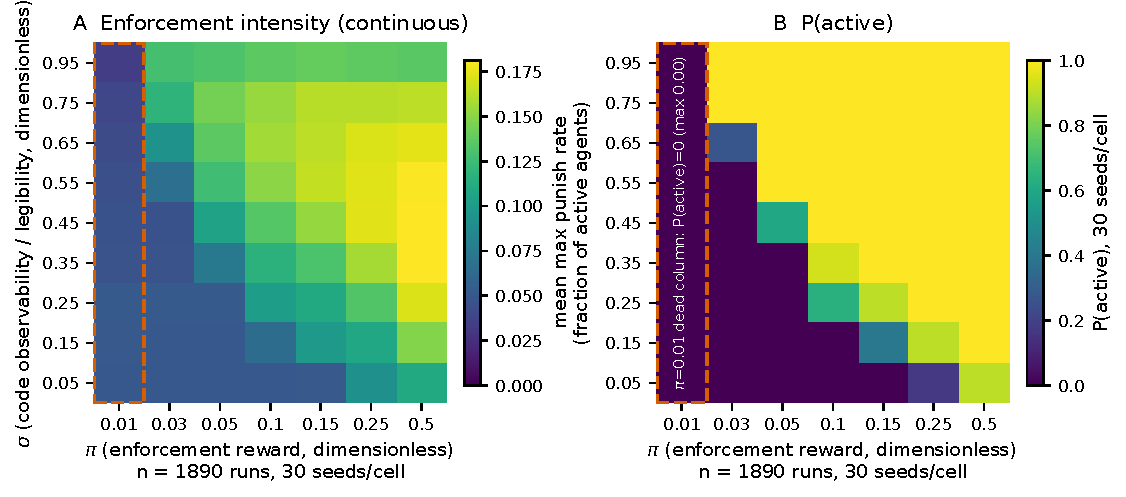
\includegraphics[width=\textwidth]{../figures/manuscript_v2/fig1_activation_frontier.pdf}
\caption{\textbf{Activation frontier under open exit.} Agent-based sweep at $\delta_0=0$ (exit open), $n=1890$ runs (9 $\sigma$ $\times$ 7 $\pi$ cells $\times$ 30 seeds per cell). (A) Mean maximum punish rate, the continuous enforcement-intensity surface. (B) Probability that a run is classified active, recomputed with the hierarchical classifier (active: max punish rate $\geq$ 0.1); overall P(active) $=$ 0.598. In the reported grid, enforcement activates only above a joint $\sigma$--$\pi$ threshold: the $\pi=0.01$ column (dashed outline) is inactive in all 9 cells, so no run in that column sustains an enforcement apparatus at any tested level of code observability.}
\label{fig:activation}
\end{figure}

\begin{figure}[htbp]
\centering
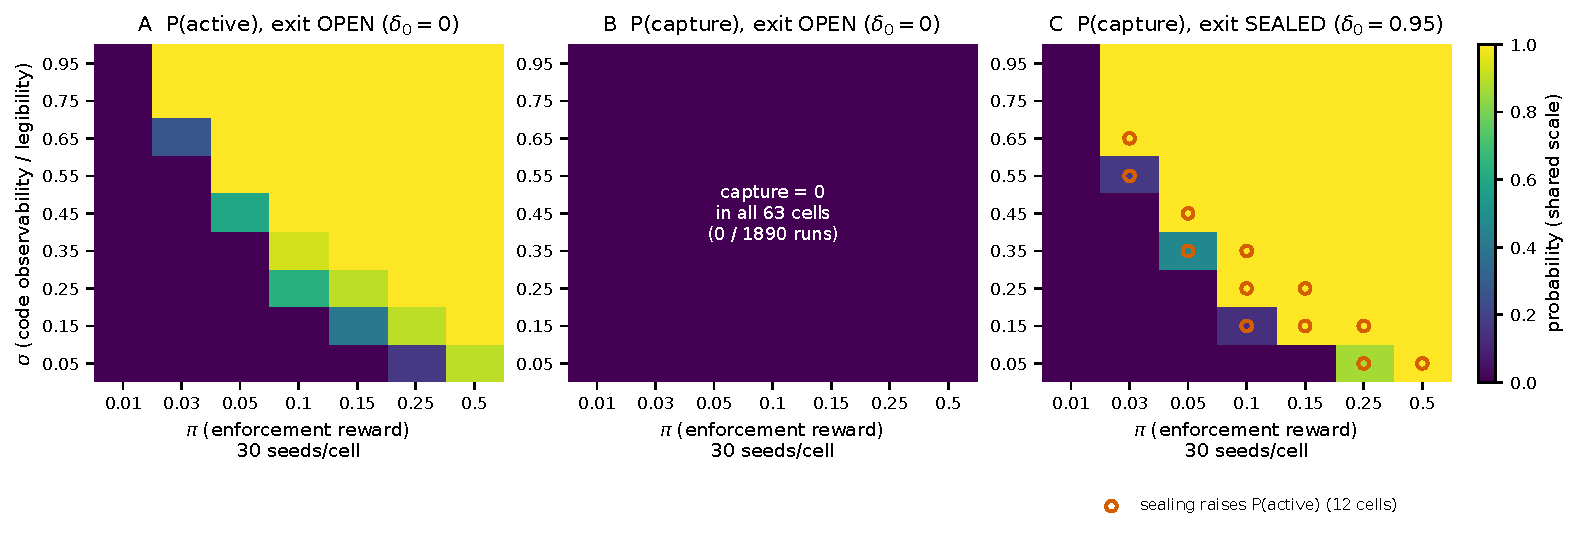
\includegraphics[width=\textwidth]{../figures/manuscript_v2/fig2_two_dimensions.pdf}
\caption{\textbf{Exit closure is necessary for capture.} All panels share one colour scale; 9 $\sigma$ $\times$ 7 $\pi$ cells $\times$ 30 seeds per cell. (A) Probability a run is active with the exit open ($\delta_0=0$, $n=1890$ runs): code geometry alone sets activation, overall P(active) $=$ 0.598. (B) Probability of capture in those same 1890 runs: \textbf{0 of 1890 runs reach capture with the exit open}; no run with the exit open reaches capture, in any of the 63 cells, despite that active rate of 0.598. (C) Probability of capture with the exit sealed ($\delta_0=0.95$, $n=1890$ runs): the active region in these runs now captures. Panels B and C are the same quantity under the two exit conditions, so the contrast isolates the effect of closing the exit. The two dimensions are not fully orthogonal: circled cells in (C) are the 12 of 63 cells where sealing also raises P(active) (mean shift over all cells +0.062; +0.328 among circled cells), and activation falls in no reported cell. Regimes recomputed with the hierarchical classifier.}
\label{fig:twodim}
\end{figure}

\begin{figure}[htbp]
\centering
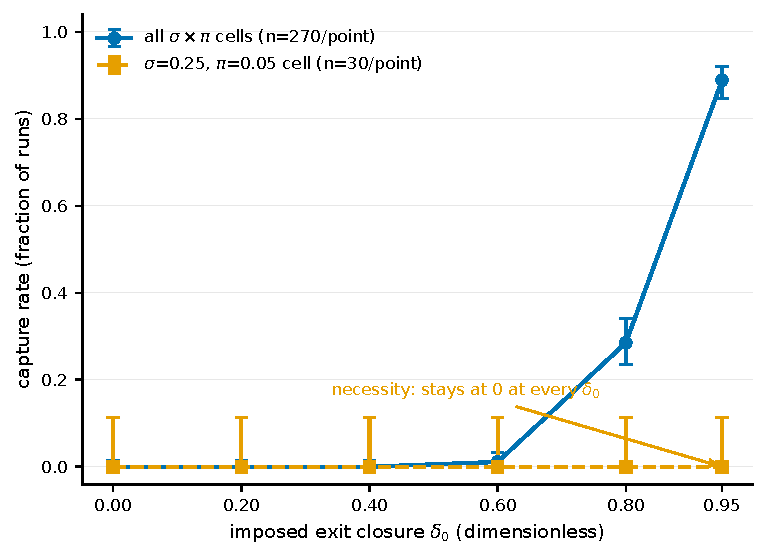
\includegraphics[width=\textwidth]{../figures/manuscript_v2/fig3_exit_closure_dose_response.pdf}
\caption{\textbf{Exit-closure dose-response and the necessity of code geometry.} Capture rate against imposed exit closure $\delta_0$ ($n=1620$ runs total; 270 runs per pooled point, 30 per cell-specific point), with Wilson 95\% intervals. Pooled over all $\sigma\times\pi$ cells (circles) capture rises monotonically from 0.000 at $\delta_0=0$ to 0.889 at $\delta_0=0.95$. In the reported runs for the $\sigma=0.25$, $\pi=0.05$ cell (squares, dashed), the capture rate is 0.000 at every tested level, including $\delta_0=0.95$: imposed closure does not produce capture in this inactive cell. Regimes recomputed with the hierarchical classifier.}
\label{fig:doseresponse}
\end{figure}

\begin{figure}[htbp]
\centering
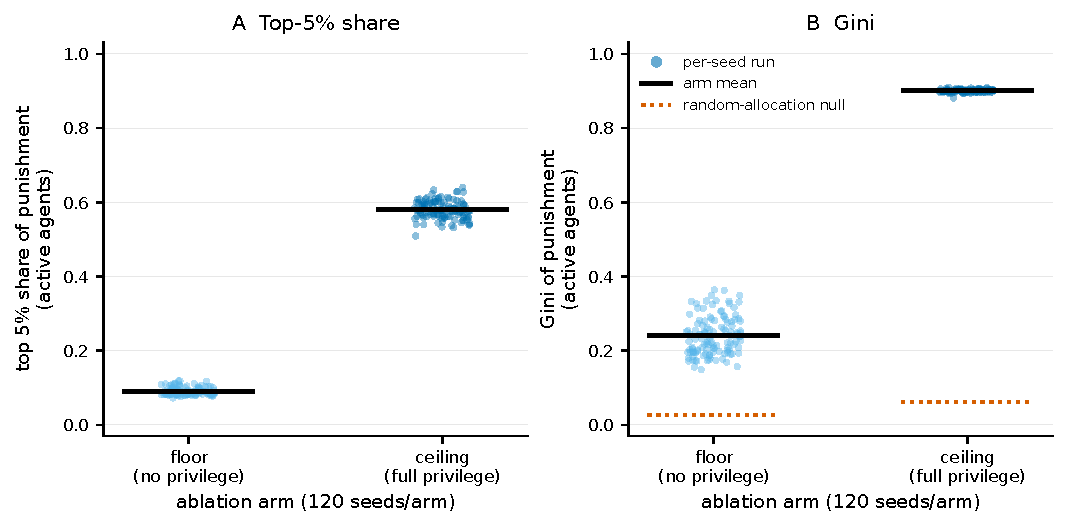
\includegraphics[width=\textwidth]{../figures/manuscript_v2/fig4_privilege_ablation.pdf}
\caption{\textbf{Concentration is manufactured by the privilege architecture.} Role-independent concentration for the ablation floor (no privilege) and ceiling (full privilege bundle), 120 seeds per arm ($n=240$ runs); points are individual runs, black bars arm means. (A) Top-5\% share of punishment among active agents rises from 0.091 at the floor to 0.580 at the ceiling, so 84\% of ceiling concentration in these runs is privilege-manufactured. (B) Gini rises from 0.240 to 0.901 against random-allocation nulls (dotted) of 0.028 and 0.062; the reported floor sits close to its null, so these runs do not show substantial concentration emerging from the unprivileged model. A committed random-allocation null exists only for the Gini statistic, so panel A carries no null reference.}
\label{fig:ablation}
\end{figure}

\section*{Acknowledgments}

% ============================================================
% REFERENCES
% ============================================================

% ============================================================
% Bibliography.
% The canonical bibliographic data live in references.bib. This
% thebibliography block is generated from that file in author-year
% form, sorted alphabetically, because bibtex is not available in
% the build environment. With bibtex present, delete the block
% below and uncomment the following line; \bibliographystyle{plainnat}
% is already set in the preamble.
%\bibliography{references}
% ============================================================
\begin{thebibliography}{43}

\bibitem[Adams(1995)]{adams1995}
Adams DW (1995) Education for Extinction: American Indians and the Boarding School Experience, 1875--1928. University Press of Kansas, Lawrence, KS.

\bibitem[Axelrod(1986)]{axelrod1986}
Axelrod R (1986) An evolutionary approach to norms. \textit{American Political Science Review} 80(4):1095--1111.

\bibitem[Berman(2000)]{berman2000}
Berman E (2000) Sect, subsidy, and sacrifice: An economist's view of ultra-Orthodox Jews. \textit{Quarterly Journal of Economics} 115(3):905--953.

\bibitem[Berman and Laitin(2008)]{bermanlaitin2008}
Berman E, Laitin DD (2008) Religion, Terrorism and Public Goods: Testing the Club Model. \textit{Journal of Public Economics} 92(10--11):1942--1967.

\bibitem[Bok(2025)]{bok2025}
Bok J (2025) Religious Exit Costs. \textit{Journal for the Scientific Study of Religion} 64(2):227--239. doi:10.1111/jssr.12963.

\bibitem[Boyd et~al.(2010)]{boydgintisbowles2010}
Boyd R, Gintis H, Bowles S (2010) Coordinated Punishment of Defectors Sustains Cooperation and Can Proliferate When Rare. \textit{Science} 328(5978):617--620. doi:10.1126/science.1183665.

\bibitem[Boyd et~al.(2003)]{boyd2003}
Boyd R, Gintis H, Bowles S, Richerson PJ (2003) The evolution of altruistic punishment. \textit{Proceedings of the National Academy of Sciences} 100(6):3531--3535.

\bibitem[Bromley(1998)]{bromley1998}
Bromley DG (1998) The Politics of Religious Apostasy: The Role of Apostates in the Transformation of Religious Movements. Praeger.

\bibitem[Carvalho(2013)]{carvalho2013}
Carvalho JP (2013) Veiling. \textit{Quarterly Journal of Economics} 128(1):337--370.

\bibitem[Carvalho(2019)]{carvalho2019}
Carvalho JP (2019) Religious Clubs: The Strategic Role of Religious Identity. In: Carvalho JP, Iyer S, Rubin J (eds) \textit{Advances in the Economics of Religion}, International Economic Association Series, vol 158. Palgrave Macmillan, Cham, pp 25--41.

\bibitem[Centola et~al.(2005)]{centola2005}
Centola D, Willer R, Macy M (2005) The emperor's dilemma: A computational model of self-enforcing norms. \textit{American Journal of Sociology} 110(4):1009--1040. doi:10.1086/427321.

\bibitem[Cook(2000)]{cook2000}
Cook M (2000) Commanding Right and Forbidding Wrong in Islamic Thought. Cambridge University Press.

\bibitem[Cragun and Hammer(2011)]{cragun2011}
Cragun RT, Hammer JH (2011) One person's apostate is another person's convert: What terminology tells us about pro-religious hegemony in the sociology of religion. \textit{Humanity \& Society} 35(1--2):149--175.

\bibitem[Engelstein(1999)]{engelstein1999}
Engelstein L (1999) Castration and the Heavenly Kingdom: A Russian Folktale. Cornell University Press, Ithaca, NY.

\bibitem[Fehr and G\"achter(2002)]{fehr2002}
Fehr E, G\"achter S (2002) Altruistic punishment in humans. \textit{Nature} 415(6868):137--140.

\bibitem[Fehr and G\"{a}chter(2000)]{fehrgachter2000}
Fehr E, G\"{a}chter S (2000) Cooperation and Punishment in Public Goods Experiments. \textit{American Economic Review} 90(4):980--994. doi:10.1257/aer.90.4.980.

\bibitem[Gelfand et~al.(2011)]{gelfand2011}
Gelfand MJ, et al (2011) Differences between tight and loose cultures: A 33-nation study. \textit{Science} 332(6033):1100--1104.

\bibitem[Given(1997)]{given1997}
Given JB (1997) Inquisition and Medieval Society: Power, Discipline, and Resistance in Languedoc. Cornell University Press.

\bibitem[Gore et~al.(2018)]{gorelemosshultswildman2018}
Gore R, Lemos C, Shults FL, Wildman WJ (2018) Forecasting Changes in Religiosity and Existential Security with an Agent-Based Model. \textit{Journal of Artificial Societies and Social Simulation} 21(1):4. doi:10.18564/jasss.3596.

\bibitem[Greif(2006)]{greif2006}
Greif A (2006) Institutions and the Path to the Modern Economy: Lessons from Medieval Trade. Cambridge University Press.

\bibitem[Greif and Mokyr(2016)]{greif2016}
Greif A, Mokyr J (2016) Cognitive rules, institutions, and economic growth: Douglass North and beyond. \textit{Journal of Institutional Economics} 13(1):25--52.

\bibitem[Harris et~al.(2020)]{numpy2020}
Harris CR, Millman KJ, van der Walt SJ, et al (2020) Array programming with NumPy. \textit{Nature} 585(7825):357--362. doi:10.1038/s41586-020-2649-2.

\bibitem[Hagberg et~al.(2008)]{networkx2008}
Hagberg AA, Schult DA, Swart PJ (2008) Exploring Network Structure, Dynamics, and Function using NetworkX. In: Varoquaux G, Vaught T, Millman J (eds) \textit{Proceedings of the 7th Python in Science Conference}, Pasadena, CA, pp 11--15.

\bibitem[Hauert et~al.(2007)]{hauertetal2007}
Hauert C, Traulsen A, Brandt H, Nowak MA, Sigmund K (2007) Via Freedom to Coercion: The Emergence of Costly Punishment. \textit{Science} 316(5833):1905--1907.

\bibitem[Hilbe et~al.(2014)]{hilbe2014}
Hilbe C, Traulsen A, R\"ohl T, Milinski M (2014) Democratic decisions establish stable authorities that overcome the paradox of second-order punishment. \textit{Proceedings of the National Academy of Sciences} 111(2):752--756.

\bibitem[Hirschman(1970)]{hirschman1970}
Hirschman AO (1970) Exit, Voice, and Loyalty: Responses to Decline in Firms, Organizations, and States. Harvard University Press.

\bibitem[Hostetler(1974)]{hostetler1974}
Hostetler JA (1974) Hutterite Society. Johns Hopkins University Press, Baltimore, MD.

\bibitem[Iannaccone(1988)]{iannaccone1988}
Iannaccone LR (1988) A Formal Model of Church and Sect. \textit{American Journal of Sociology} 94(Supplement):S241--S268. doi:10.1086/228948.

\bibitem[Iannaccone(1992)]{iannaccone1992}
Iannaccone LR (1992) Sacrifice and Stigma: Reducing Free-Riding in Cults, Communes, and Other Collectives. \textit{Journal of Political Economy} 100(2):271--291.

\bibitem[Iannaccone(1994)]{iannaccone1994}
Iannaccone LR (1994) Why Strict Churches Are Strong. \textit{American Journal of Sociology} 99(5):1180--1211.

\bibitem[Iannaccone and Makowsky(2007)]{iannacconemakowsky2007}
Iannaccone LR, Makowsky MD (2007) Accidental Atheists? Agent-Based Explanations for the Persistence of Religious Regionalism. \textit{Journal for the Scientific Study of Religion} 46(1):1--16.

\bibitem[Iyer(2016)]{iyer2016}
Iyer S (2016) The New Economics of Religion. \textit{Journal of Economic Literature} 54(2):395--441. doi:10.1257/jel.54.2.395.

\bibitem[Kazil et~al.(2020)]{mesa2020}
Kazil J, Masad D, Crooks A (2020) Utilizing Python for Agent-Based Modeling: The Mesa Framework. In: Thomson R, Bisgin H, Dancy C, Hyder A, Hussain M (eds) \textit{Social, Cultural, and Behavioral Modeling}, Lecture Notes in Computer Science, vol 12268. Springer, Cham, pp 308--317. doi:10.1007/978-3-030-61255-9\_30.

\bibitem[Kelly(1989)]{kelly1989}
Kelly HA (1989) Inquisition and the prosecution of heresy: Misconceptions and abuses. \textit{Church History} 58(4):439--451.

\bibitem[Kuran(1995)]{kuran1995}
Kuran T (1995) Private Truths, Public Lies: The Social Consequences of Preference Falsification. Harvard University Press.

\bibitem[Mann(1986)]{mann1986}
Mann M (1986) The Sources of Social Power, Vol. 1. Cambridge University Press.

\bibitem[McBride(2007)]{mcbride2007}
McBride M (2007) Club Mormon: Free-Riders, Monitoring, and Exclusion in the LDS Church. \textit{Rationality and Society} 19(4):395--424. doi:10.1177/1043463107083736.

\bibitem[McKinney(2010)]{pandas2010}
McKinney W (2010) Data Structures for Statistical Computing in Python. In: van der Walt S, Millman J (eds) \textit{Proceedings of the 9th Python in Science Conference}, pp 56--61. doi:10.25080/Majora-92bf1922-00a.

\bibitem[Norenzayan and Gervais(2013)]{norenzayan2013}
Norenzayan A, Gervais WM (2013) The origins of religious disbelief. \textit{Trends in Cognitive Sciences} 17(1):20--25.

\bibitem[North(1990)]{north1990}
North DC (1990) Institutions, Institutional Change and Economic Performance. Cambridge University Press.

\bibitem[Pierson(2000)]{pierson2000}
Pierson P (2000) Increasing returns, path dependence, and the study of politics. \textit{American Political Science Review} 94(2):251--267.

\bibitem[Rubin(2017)]{rubin2017}
Rubin J (2017) Rulers, Religion, and Riches: Why the West Got Rich and the Middle East Did Not. Cambridge University Press.

\bibitem[Scott(1998)]{scott1998}
Scott JC (1998) Seeing Like a State: How Certain Schemes to Improve the Human Condition Have Failed. Yale University Press.

\bibitem[Sigmund et~al.(2010)]{sigmund2010}
Sigmund K, De Silva H, Traulsen A, Hauert C (2010) Social learning promotes institutions for governing the commons. \textit{Nature} 466(7308):861--863.

\bibitem[Streib et~al.(2009)]{streib2009}
Streib H, Hood RW, Keller B, Cs\"off RM, Silver CF (2009) Deconversion: Qualitative and Quantitative Results from Cross-Cultural Research in Germany and the United States of America. Vandenhoeck \& Ruprecht.

\bibitem[Tilly(1985)]{tilly1985}
Tilly C (1985) War making and state making as organized crime. In: Evans P, Rueschemeyer D, Skocpol T (eds) \textit{Bringing the State Back In}. Cambridge University Press, pp 169--191.

\bibitem[Weber(1946)]{weber1946}
Weber M (1946) Politics as a Vocation. In: Gerth HH, Mills CW (eds) \textit{From Max Weber: Essays in Sociology}. Oxford University Press, pp 77--128. (Original work published 1919.)

\bibitem[Wildman and Sosis(2011)]{wildmansosis2011}
Wildman WJ, Sosis R (2011) Stability of Groups with Costly Beliefs and Practices. \textit{Journal of Artificial Societies and Social Simulation} 14(3):6. doi:10.18564/jasss.1781.

\end{thebibliography}

\section*{Data and Code Availability}

All simulation code, data, and analysis scripts are publicly available: an anonymized review copy of the repository is available at [ANONYMOUS-LINK]; the public archive will be linked upon acceptance.

\section*{Supporting Information}

\noindent\textbf{Online Resource 1.} Supporting text covering the parameter-to-observable mapping, the complete model-parameter tables, classification robustness including the activation-threshold sensitivity, the continuous observability--reward and closure surfaces, the privilege ablation, the endogenous exit-capacity analysis with its anti-circularity test, and computational reproducibility with the committed-run inventory.

\end{document}
